\section{Physics Requirements}

\subsection{Performance criteria}
The design parameters of the PCAL were established using the full GEANT simulations of the PCAL-EC system. These studies are described in detail in Refs. \cite{2007001} and are summarized below. The mechanical design depends on the number of scintillator-lead layers, on the angular coverage of the PCAL, and on the size of the readout segmentation. These parameters were determined by the physics requirements for the detection and identification of high energy electrons, photons, and $\pi^{0}$ meson via $2\gamma$\ decay.

\begin{figure}[hbt]
\centering
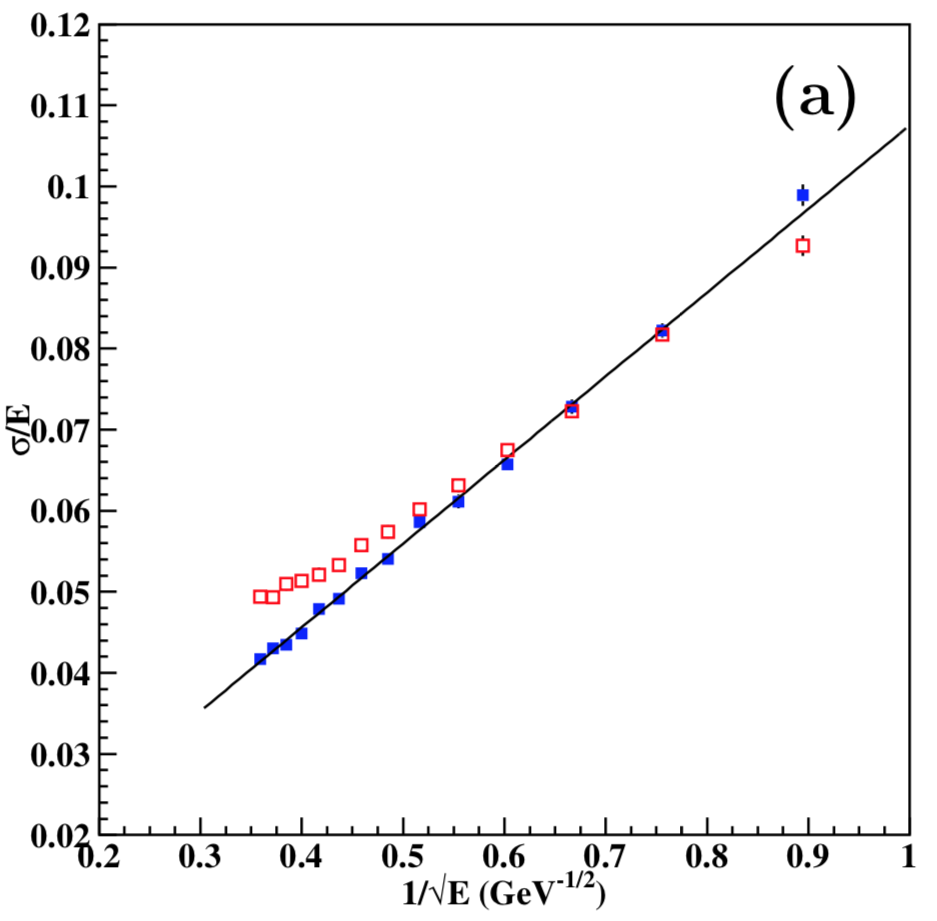
\includegraphics[width=0.85\columnwidth,keepaspectratio]{img/S2_1_a.png}
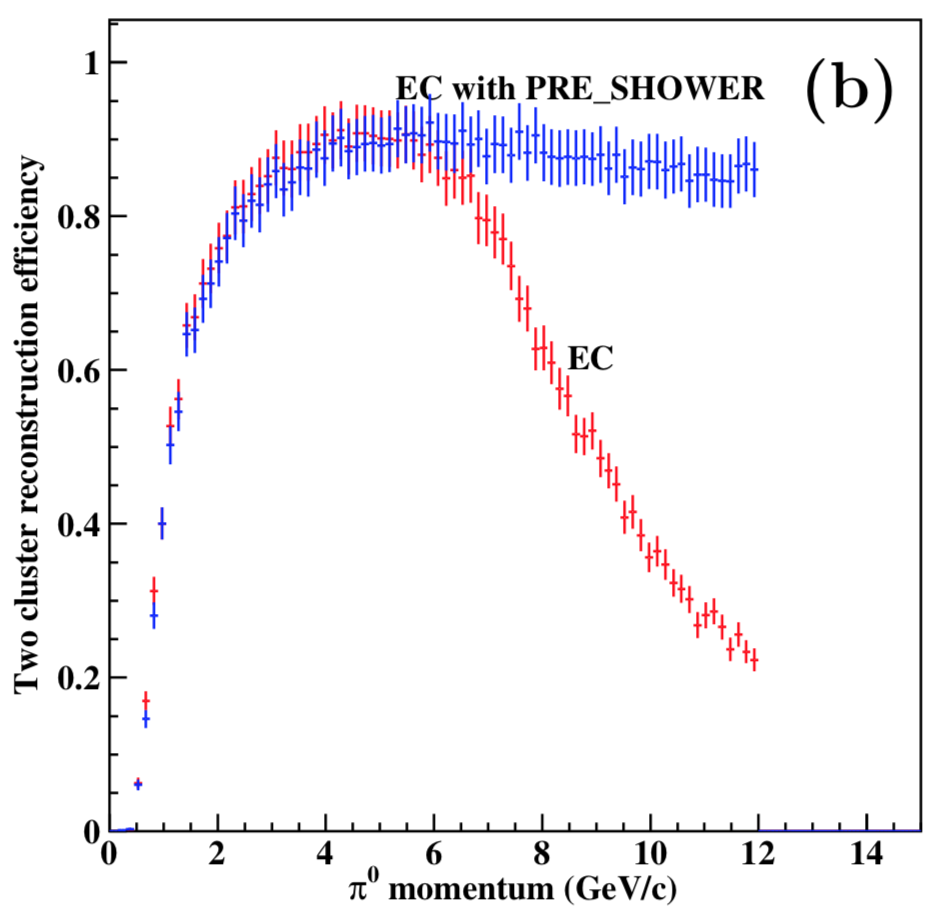
\includegraphics[width=0.85\columnwidth,keepaspectratio]{img/S2_1_b.png}
\caption[Simulated performance]{Comparison of simulated performance of combined PCAL+EC calorimeter (blue points) and EC only (red points) at CLAS12 energies. a) Energy resolution as a function of inverse square root of energy. b) Reconstruction efficiency of two clusters from $\pi^{0}$ decay photons as a function of pion momentum.}
\label{fig:S2_1}
\end{figure}

Initial simulations were carried out with 15 layers of lead and scintillator (similar to the inner part of the EC), using 35 mm wide segmentation for the scintillator layers, corresponding to about 108 readout channels in each stereo view. For comparison the EC uses 100 mm wide strips.  Events were generated in a uniform distribution of  $\pi^{0}$ and photon events at the target with momenta up to 12 GeV/c. Reconstruction of clusters was done using the standard cluster reconstruction algorithm of the EC, but applied to both PCAL and EC. As shown in Fig. \ref{fig:S2_1}, the combined PCAL and EC system retains good energy resolution, $\sigma/E \approx 0.1 \times E^{-1/2}$, and constant efficiency for two cluster reconstruction up to the highest momenta.

Additional simulations were performed using variable segmentation of the scintillator layers. Keeping constant the total number of readout channels per sector, it was found that maximum efficiency can be obtained if half of each stereo layer is equipped with 45 mm wide strips and half with 90 mm wide strips (double strip readout). The triangular stereo layers overlap such that there is always a region with 45 mm wide strips in one of the stereo layers, as shown in Fig. \ref{fig:S2_2}. There is only a small loss of two-cluster efficiency at the highest momenta for this geometry compared with 45 mm wide strips in all stereo layers. It should be noted that at forward angles (short U-strips) where most of the high energy $\pi^{0}$ are produced all three stereo readout views have small readout segmentation.

\begin{figure}[hbt]
\centering
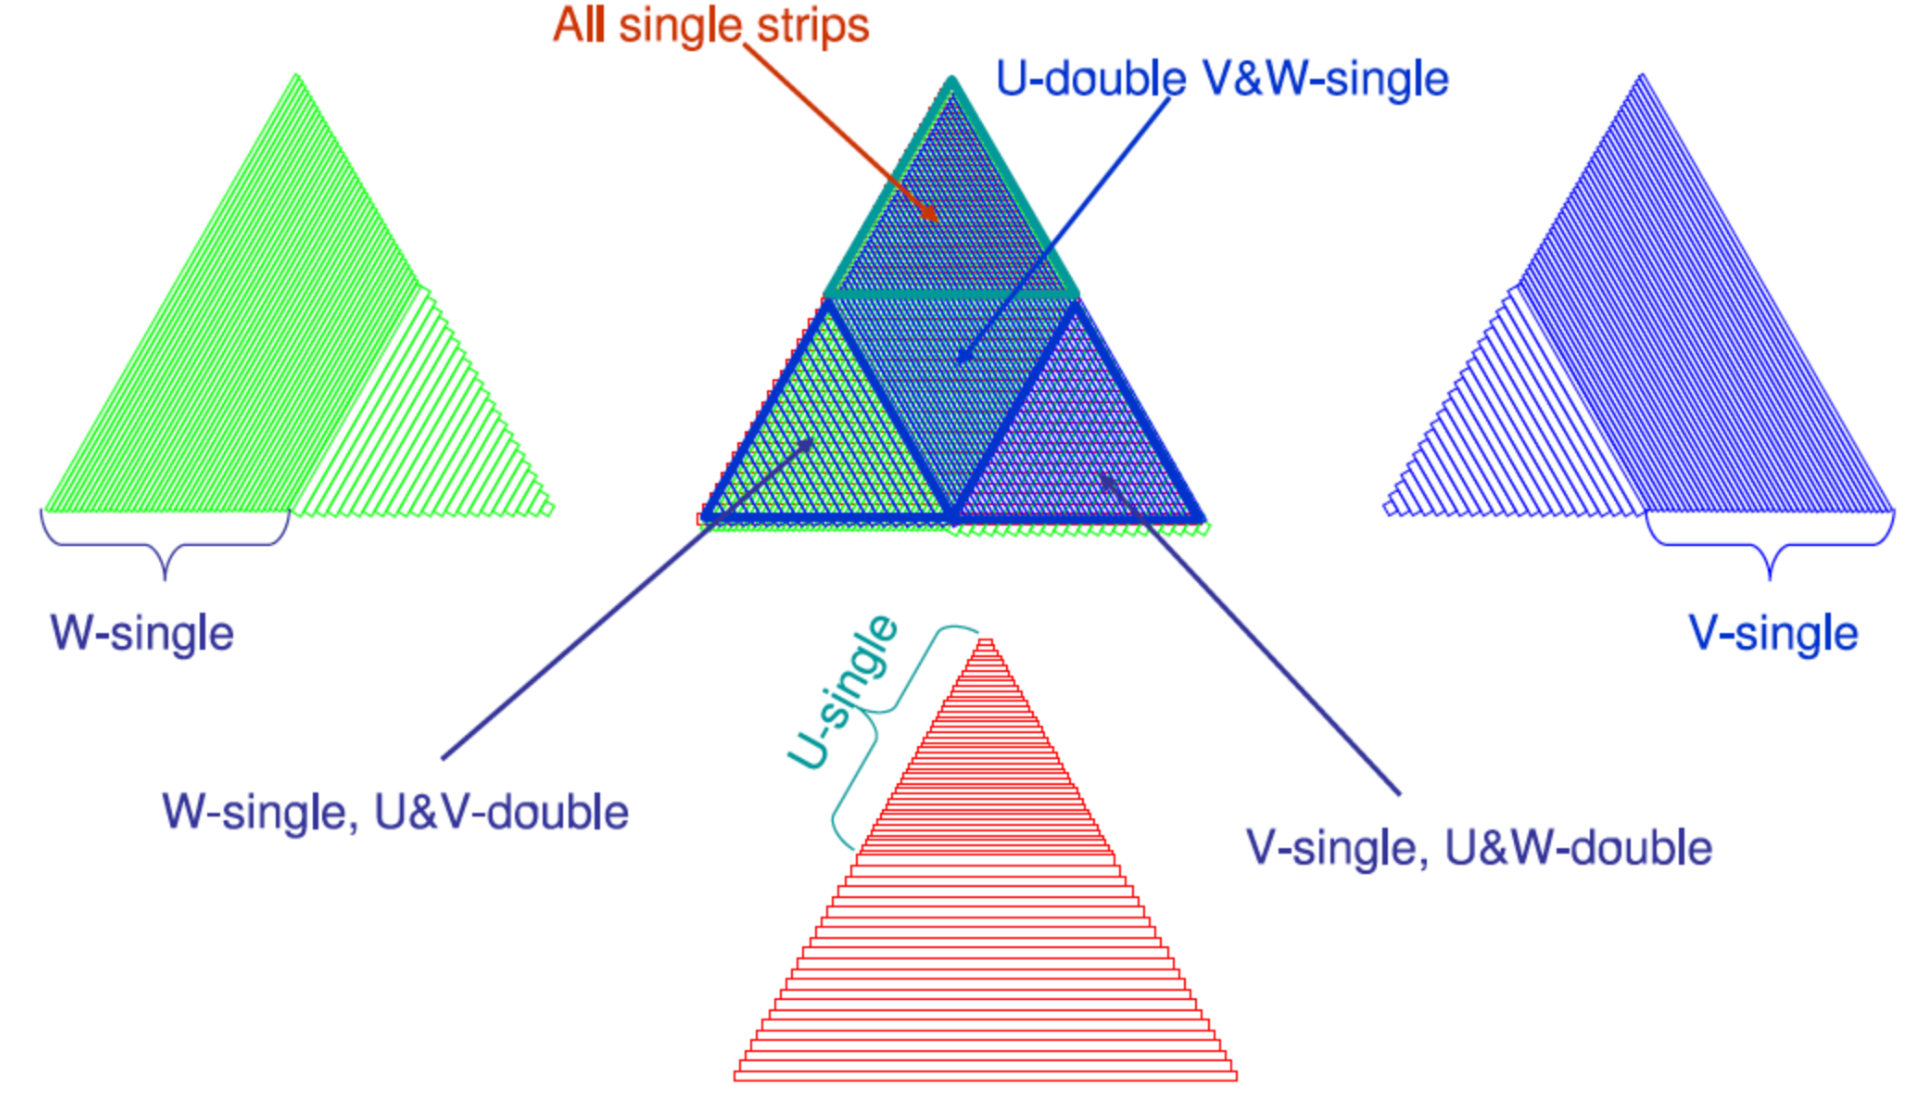
\includegraphics[width=0.95\columnwidth,keepaspectratio]{img/S2_2.png}
\caption{Segmentation pattern for different stereo readout planes (U, V, and W). There is always a region with single strip width (45 mm) readout in one of the stereo layers.  The U PMTs are readout from the left side of the triangle, as seen in this view from the target, while the V and W PMTs are readout from the base.}
\label{fig:S2_2}
\end{figure}



